\documentclass[14pt]{beamer}


\usepackage{color}
\usepackage{tikz}


\mode<presentation>
{
\usetheme{AlpesLasers}
\setbeamercovered{transparent}
  %\setbeamertemplate{footline}[frame number] 
  %\setbeamertemplate{navigation symbols}{ 
  %\hskip 0.3cm
  %\insertframenumber / \inserttotalframenumber  % <<< frame #
  %\insertpagenumber / \insertpresentationendpage % <<< page #
%} 
}

% font definitions, try \usepackage{ae} instead of the following
% three lines if you don't like this look
\usepackage{listings}
\lstloadlanguages{python}

\usepackage{mathptmx}
\usepackage[scaled=.90]{helvet}
\usepackage{courier}
\usepackage[T1]{fontenc}
\usepackage[english]{babel}
\usepackage[latin1]{inputenc}
\title{Why PYTHON is THE computer language for physicists}
\subtitle{Libraries, usage examples}
\author{St\'ephane Poss}
\date{\today}
% This is only inserted into the PDF information catalog. Can be left
% out.
\subject{PYTHON}

\lstdefinestyle{custompy}{
  belowcaptionskip=1\baselineskip,
  breaklines=true,
  xleftmargin=\parindent,
  language=python,
  showstringspaces=false,
  basicstyle=\footnotesize\ttfamily,
  keywordstyle=\bfseries\color{green!40!black},
  commentstyle=\itshape\color{purple!40!black},
  identifierstyle=\color{blue},
  stringstyle=\color{orange},
}
\lstdefinestyle{customsh}{
  belowcaptionskip=1\baselineskip,
  breaklines=true,
  xleftmargin=\parindent,
  language=bash,
  showstringspaces=false,
  basicstyle=\footnotesize\ttfamily,
  keywordstyle=\bfseries\color{green!40!black},
  commentstyle=\itshape\color{purple!40!black},
  identifierstyle=\color{blue},
  stringstyle=\color{orange},
}
\lstdefinestyle{customcpp}{
  belowcaptionskip=1\baselineskip,
  breaklines=true,
  xleftmargin=\parindent,
  language=C++,
  showstringspaces=false,
  basicstyle=\footnotesize\ttfamily,
  keywordstyle=\bfseries\color{green!40!black},
  commentstyle=\itshape\color{purple!40!black},
  identifierstyle=\color{blue},
  stringstyle=\color{orange},
}

\begin{document}
\begin{frame}[plain]
\titlepage
\end{frame}

\begin{frame}
\tableofcontents
\end{frame}

\section{IPython}
\begin{frame}
\frametitle{IPython}
\begin{columns}
\column{0.69\textwidth}
\begin{itemize}
\item Command shell 
\item Tab completion
\item Web browser interface (notebook)
\item Tools for parallel computing
\end{itemize}
\column{0.39\textwidth}

\includegraphics[width=\textwidth]{IPython_Logo.png}
\end{columns}
~\\
\url{http://www.ipython.org}
\end{frame}

\section{Libraries for physicist}

\subsection{NumPy}
\begin{frame}
\frametitle{NumPy}
\begin{columns}
\column{0.69\textwidth}
\begin{itemize}
\item Adds support for large N-dim arrays and matrices
\item Large library of math functions
\item FFT, Linear alg, rng
\item Interface with C++/fortran
\item Close to MATLAB
\end{itemize}
\column{0.39\textwidth}

\includegraphics[width=\textwidth]{NumPy_logo.png}
\end{columns}
~\\
\url{http://www.numpy.org}
\end{frame}

\begin{frame}
\frametitle{NumPy example}
\lstinputlisting[style=custompy]{numpyex.py}
\end{frame}

\subsection{SciPy}
\begin{frame}
\frametitle{SciPy}
\begin{columns}
\column{0.69\textwidth}
\begin{itemize}
\item Goes with NumPy
\item Optimization
\item Interpolation
\item FFT
\item Image processing
\item Numerical integral
\item Diff. equation solving
\item Statistics
\end{itemize}
\column{0.39\textwidth}

\includegraphics[width=\textwidth]{Scipylogo.png}
\end{columns}
~\\
\url{http://www.scipy.org}
\end{frame}

\begin{frame}
\frametitle{SciPy Linear Alg. example}
\lstinputlisting[style=custompy]{scipy.py}
\end{frame}

\begin{frame}
\frametitle{SciPy FFT example}
\lstinputlisting[style=custompy]{scipy2.py}
\end{frame}

\begin{frame}
\frametitle{SciPy FFT example}
\lstinputlisting[style=custompy]{scipy3.py}
\end{frame}

\subsection{Matplotlib}
\begin{frame}
\frametitle{Matplotlib}
\begin{columns}
\column{0.69\textwidth}
\begin{itemize}
\item Integrates with NumPy, SciPy
\item Produces plots
\end{itemize}
\column{0.49\textwidth}
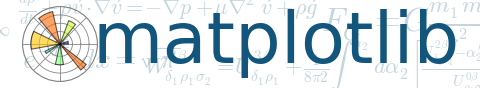
\includegraphics[width=\textwidth]{matplotlib_logo.png}
\end{columns}
~\\
\url{http://www.matplotlib.org}
\end{frame}

\begin{frame}
\frametitle{Matplotlib examples}
\begin{columns}
\column{0.49\textwidth}
\lstinputlisting[style=custompy]{matpl1.py}
\column{0.69\textwidth}
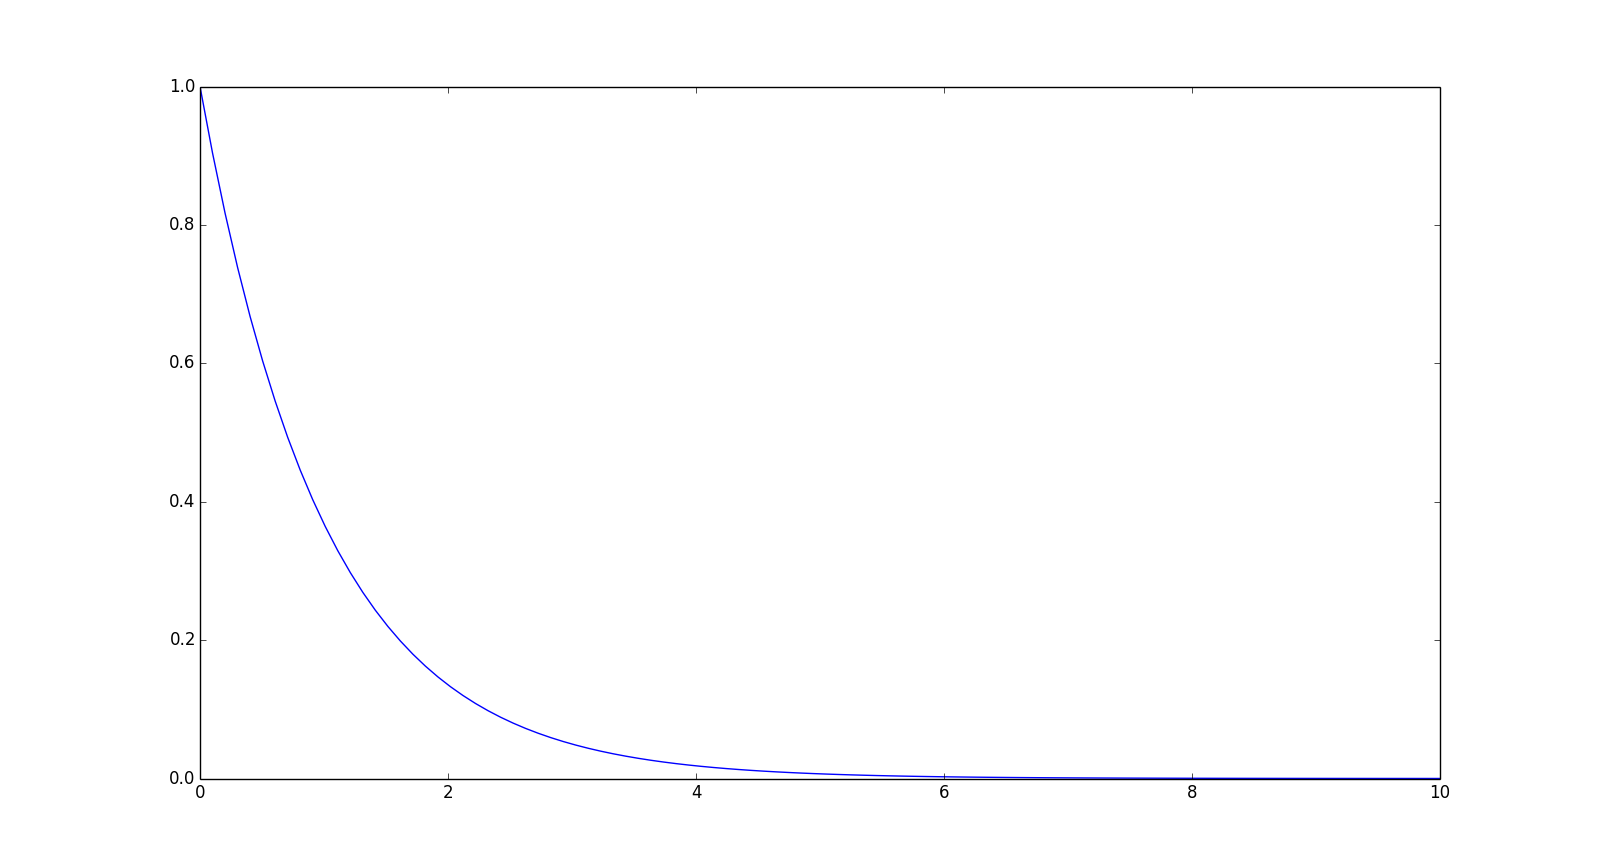
\includegraphics[width=\textwidth]{Matplotlib_basic.png}
\end{columns}
\end{frame}

\begin{frame}
\frametitle{Matplotlib examples}
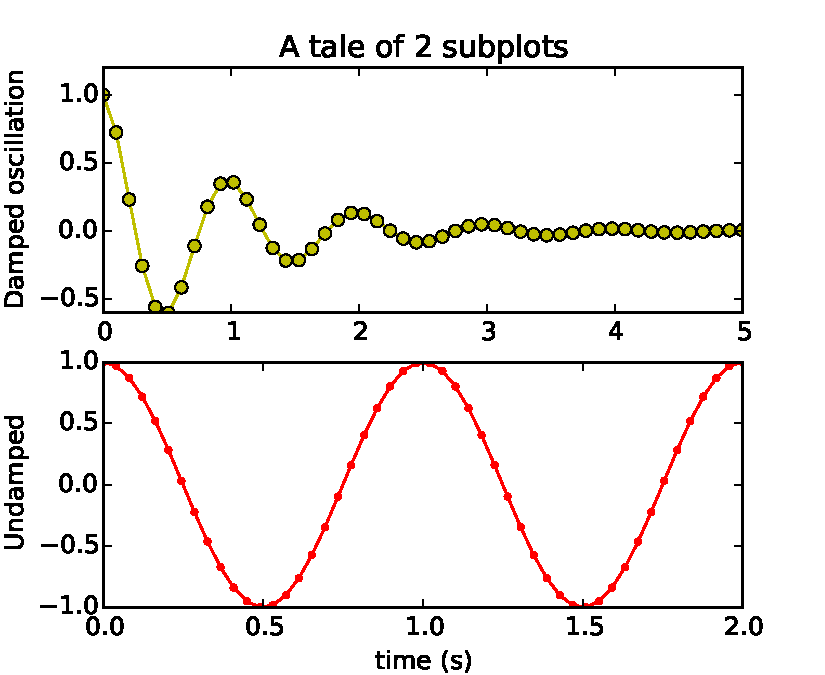
\includegraphics[width=\textwidth]{subplot_demo.pdf}
\end{frame}

\begin{frame}
\frametitle{Matplotlib examples}
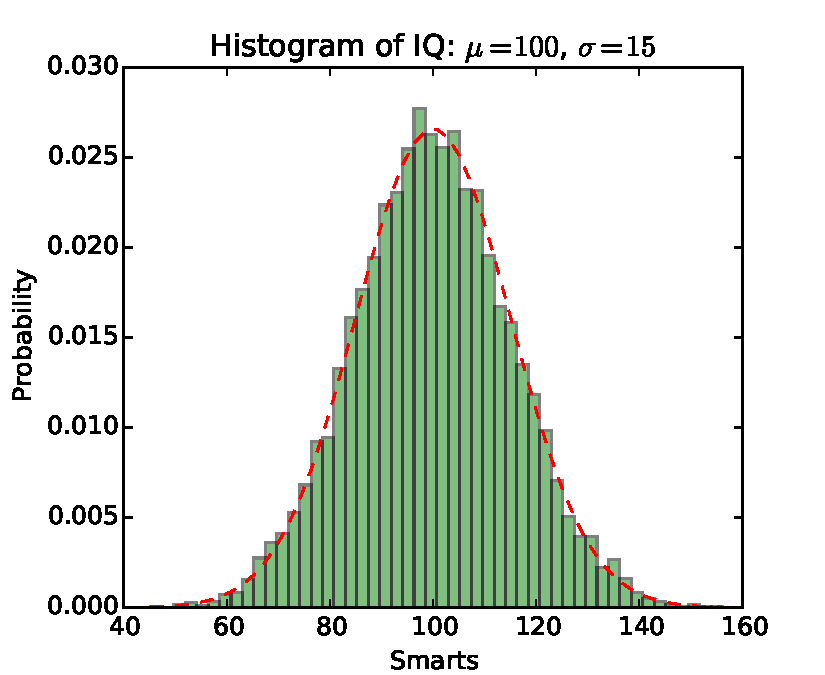
\includegraphics[width=\textwidth]{histogram_demo_features.pdf}
\end{frame}

\begin{frame}
\frametitle{Matplotlib examples}
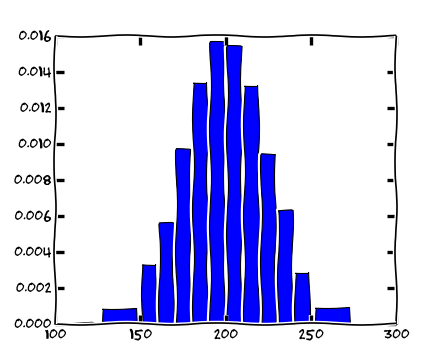
\includegraphics[width=\textwidth]{histogram_demo_extended_01.png}
\end{frame}

\begin{frame}
\frametitle{Alternative: PyQtGraph}
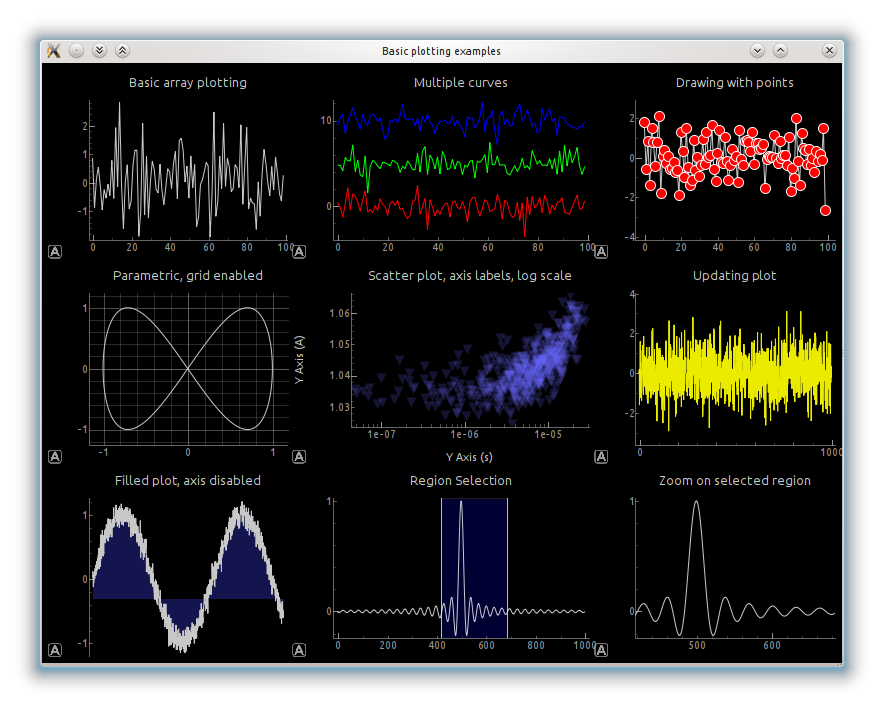
\includegraphics[width=\textwidth]{plotting_pyqtgraph.png}\\
Based on Qt.
\end{frame}

\subsection{SymPy}
\begin{frame}
\frametitle{SymPy}
\begin{columns}
\column{0.69\textwidth}
\begin{itemize}
\item Symbolic computation
\item differentiate, integrate, etc.
\item limits
\item equ. solver
\item many other things
\end{itemize}
\column{0.49\textwidth}

\includegraphics[width=\textwidth]{sympy.png}
\end{columns}
~\\
\url{http://www.sympy.org}
\end{frame}

\begin{frame}
\frametitle{SymPy examples}
\lstinputlisting[style=custompy]{sympy2.py}
\end{frame}

\begin{frame}
\frametitle{SymPy examples}
\lstinputlisting[style=custompy]{sympy3.py}
\end{frame}


\subsection{Scikit-learn}
\begin{frame}
\frametitle{Scikit-learn}
\begin{columns}
\column{0.69\textwidth}
\begin{itemize}
\item Machine learning
\item Classification
\item Regression
\item Clustering
\item And more
\end{itemize}
\column{0.49\textwidth}

\includegraphics[width=\textwidth]{scikit-learn-logo-small.png}
\end{columns}
~\\
\url{http://scikit-learn.org/stable/}
\end{frame}

\begin{frame}
\frametitle{Scikit-learn}
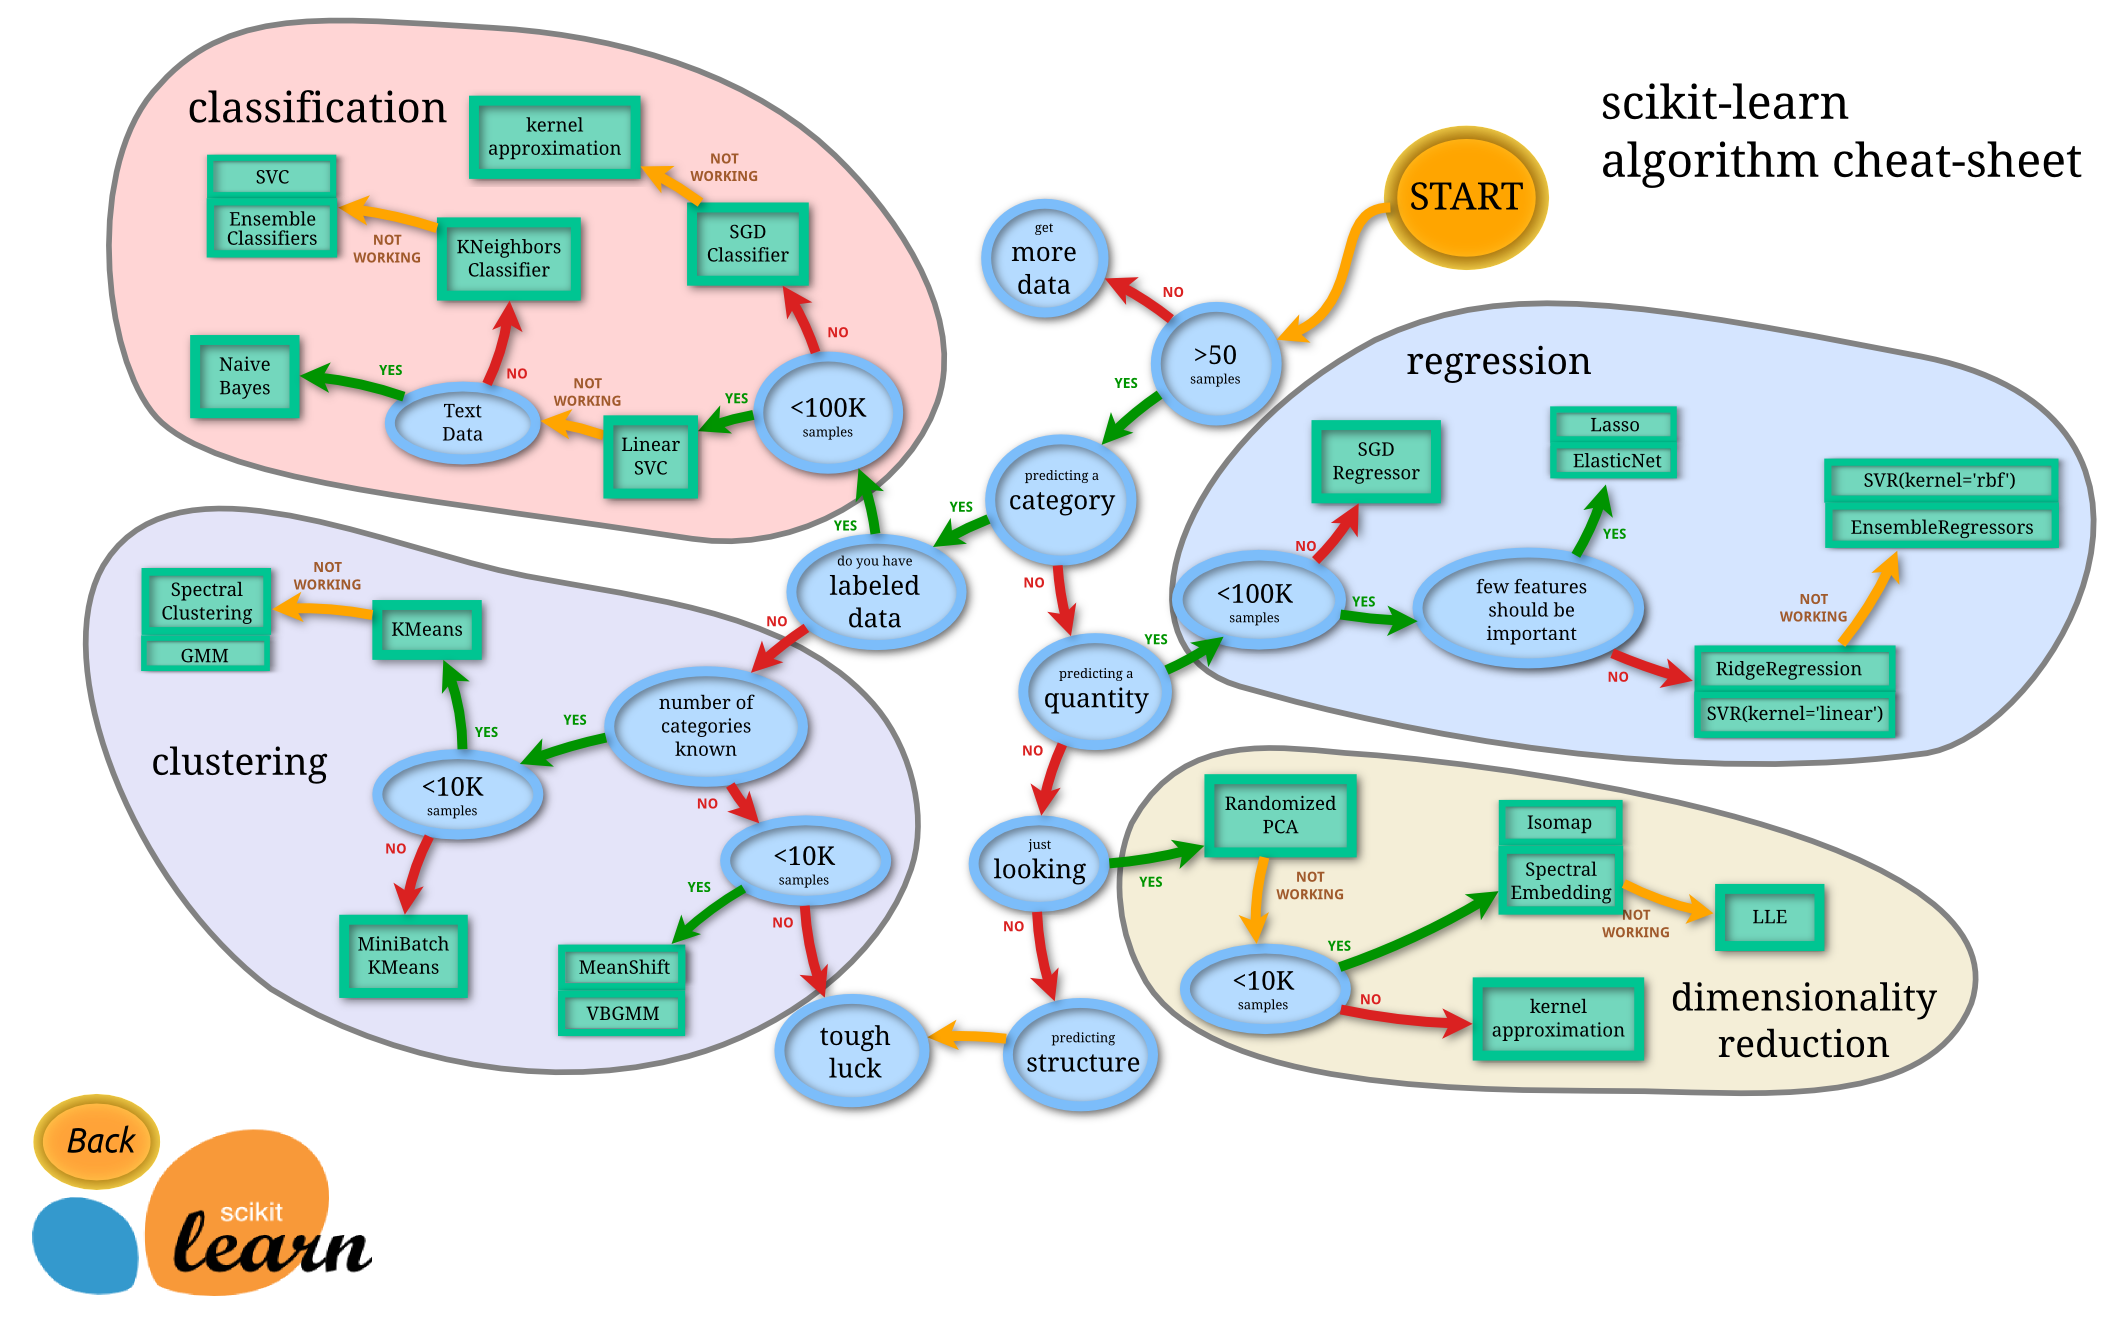
\includegraphics[width=\textwidth]{ml_map.png}
\end{frame}

\subsection{Pandas}
\begin{frame}
\frametitle{Pandas}
\begin{columns}
\column{0.49\textwidth}
\begin{itemize}
\item Data analysis
\item Similar to R
\item On top of NumPy
\end{itemize}
\column{0.69\textwidth}
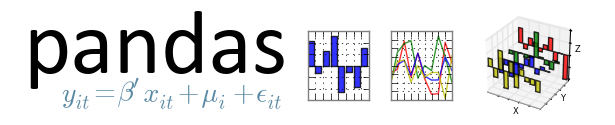
\includegraphics[width=\textwidth]{pandas_logo.png}
\end{columns}
~\\
\url{http://pandas.pydata.org/}
\end{frame}

\subsection{AstroPy}
\begin{frame}
\frametitle{AstroPy}
\begin{columns}
\column{0.59\textwidth}
\begin{itemize}
\item Dedicated to astronomers
\item Lots of utilities
\item Access to common databases
\item Standard Astro I/O
\item Modelization capabilities
\end{itemize}
\column{0.69\textwidth}

\includegraphics[width=\textwidth]{astropy_banner_96.png}
\end{columns}
~\\
\url{http://www.astropy.org/}
\end{frame}


\subsection{Cython}
\begin{frame}
\frametitle{Cython}
\centering

\includegraphics[width=3cm]{Cython-logo.png}
\begin{itemize}
\item If speed is an issue
\item Produces C compiled code
\item Adds explicit typing
\item Very efficient with NumPy arrays
\item Still PYTHON code!
\end{itemize}
\end{frame}

\begin{frame}
\frametitle{Summary}
\begin{itemize}
\item Many libraries are available to solve common physics studies problems
\item Certainly missed a few
\item All those presented here have huge documentation
\end{itemize}
\alert{Already largely used in scientific communities}
\end{frame}

\section{Use examples}

\begin{frame}
\frametitle{Astronomers}
\begin{itemize}
\item First real users of PYTHON
\item Numpy
\item AstroPy
\item Many current experiments/satellites use it: e.g. Fermi-LAT
\end{itemize}
\end{frame}

\begin{frame}
\frametitle{CERN}
\begin{itemize}
\item ATLAS/LHCb use GAUDI.
\item GAUDI uses PYTHON for its configuration
\item Trigger systems are configured using Python
\item More and more support is given to PYTHON made analysis
\end{itemize}
\end{frame}

\section{Conclusion}
\begin{frame}
\frametitle{Conclusion}
\begin{itemize}
\item Widely used in the world
\item Already adopted in the scientific community
\item Can be more efficient than other languages
\item \alert{Why not adopting it?}
\end{itemize}
\end{frame}

\appendix
\section{Bibliography}

\begin{frame}
\frametitle{Bibliography}
\url{http://scipy-lectures.github.io/}\\
Python pocket reference\\ (O'Reilly ISBN-13: 978-1449357016)\\
Head First Python\\ (O'Reilly ISBN-13: 978-1449382674)\\
Learning IPython for Interactive Computing and Data Visualization \\(ISBN 978-1-78216-993-2)
\end{frame}

\end{document}